\section{System Explanation}
\label{ch2:sec:system-explanation}

% REMARK: Put picture somewhere else
% REMARK: Shorten summary

\begin{figure}[htb]\centering
% Define some block styles
\tikzstyle{box} = [%
	draw,%
	rectangle,%
	%fill=green!20,%
	minimum height=3em,%
	minimum width=5em,%
]
\subfloat[]{%
	\begin{tikzpicture}[node distance=1.5cm, shorten >= 1pt, >=stealth', auto, scale=0.8, transform shape]
		% Define nodes
	    \path (0,0)
	    node [box, fill=blue!20](data) {Data}
	    node [box, fill=blue!20, below of=data](forecast) {Forecast}
	    node [box, fill=blue!20, below of=forecast](schedule) {Schedule}
	    node [box, below of=schedule](battery) {Battery}
	    node [box, below of=battery](network) {Network};
		% Draw lines
		\draw [->] (data) to (forecast);
		\draw [->] (forecast) to (schedule);
		\draw [->] (schedule) to (battery);
		\draw [->] (battery) to (network);
	\end{tikzpicture}%
	\label{ch2:subfig:traditional-forecast-based-system}%
}
\hspace{10mm}
\subfloat[]{
	\begin{tikzpicture}[node distance=1.5cm, shorten >= 1pt, >=stealth', auto, scale=0.8, transform shape]
		% Define nodes
	    \path
	    (0,0) 
	   	node [box, fill=green!20, below of=schedule, xshift=-14.5mm](controller) {Controller}
		node [box, fill=green!20, below of=controller](mpc) {MCP}
	    node [box, right of=controller, xshift=15mm](battery) {Battery}
	    node [box, below of=battery](network) {Network};;
		% Draw lines
		\draw [->] (network) to (mpc);
		\draw [->] (mpc) to (controller);
		\draw [->] (controller) to (battery);
		\draw [->] (battery) to (network);
	\end{tikzpicture}%
	\label{ch2:subfig:traditional-on-line-system}%
}
\hspace{10mm}
\subfloat[]{%
	\begin{tikzpicture}[node distance=1.5cm, shorten >= 1pt, >=stealth', auto, scale=0.8, transform shape]
		% Define nodes
	    \path
	    (0,0)
	    node [box, fill=blue!20](data) {Data}
	    node [box, fill=blue!20, below of=data](forecast) {Forecast}
	    node [box, fill=blue!20, below of=forecast](schedule) {Schedule}
	    node [box, below of=schedule](battery) {Battery}
	    node [box, below of=battery](network) {Network}
	   	node [box, fill=green!20, left of=battery, xshift=-14.5mm](controller) {Controller}
		node [box, fill=green!20, below of=controller](mpc) {MCP};
		% Draw lines
		\draw [->] (data) to (forecast);
		\draw [->] (forecast) to (schedule);
		\draw [->, bend right] (schedule.180) to (controller.90);
		\draw [->] (network) to (mpc);
		\draw [->] (mpc) to (controller);
		\draw [->] (controller) to (battery);
		\draw [->] (battery) to (network);
	\end{tikzpicture}%
	\label{ch2:subfig:proposed-hybrid-system}%
}

\caption{Combination of traditional forecast driven BESS control (Subfig. \ref{ch2:subfig:traditional-forecast-based-system}) and traditional on-line system (Subfig. \ref{ch2:subfig:traditional-on-line-system}) results in the proposed hybrid system (Subfig. \ref{ch2:subfig:proposed-hybrid-system}).}
\label{ch2:fig:system-diagram}
\end{figure}


The presented work was part of the \textit{New Thames Valle Vision} (NTVV) research project, and was conducted in collaboration with the British DNO \textit{Scottish and Southern Energy Networks} (SSEN) \cite{NTVV2016}.
From the findings of this research project, the diagram in Figure \ref{ch2:fig:system-diagram} was generated, showing two well established BESS control approaches and the proposed dynamic control approach.
In this figure, all constituent systems are included that were used during the BESS street-level deployment.
The two traditional systems are off-line and on-line BESS control, which are shown in Figure \ref{ch2:subfig:traditional-forecast-based-system} and \ref{ch2:subfig:traditional-on-line-system}, respectively.
Alongside these two control approaches is the proposed dynamic control system, shown in Figure \ref{ch2:subfig:proposed-dynamic-control-system}.
This control approach entails the benefits from both the traditional forecast driven and the on-line BESS control system, and is hence referred to as the hybrid of the two traditional approaches.
Unlike previous work however, this hybrid does not use Set-Point Control (SPC), which is aided by a MPC to compensate for trends in the load profile.
Instead, it operates by executing a predetermined BESS schedule with real-time adjustments, which are based on MPC-guided instructions.
Details about this control are outlined in Section \ref{ch2:sec:control-of-bess}.

In this section however, the battery model, which is used in this work is explained first.
Also the load data acquisition, forecasting and BESS schedule generation are outlined, where scheduling is performed in accordance to the BESS model's constraints.

\subsection{BESS model}

\nomenclature{$C_{bat}$}{Battery capacity in kWh, where $C_{bat} \in \mathbb{Z}^{>0}$}
\nomenclature{$C_{f}$}{Charge factor or ``C-factor'' of the battery, where $C_{f} \in \mathbb{Z}^{>0}$}
\nomenclature{$\eta$}{Self-discharge losses of battery, where $\eta \in (0, 1)$}
\nomenclature{$P_{bat}$}{BESS power electronic rating, where $P_{bat} \in \mathbb{Z}^{>0}$}
\nomenclature{$\mu$}{Round-trip efficiency of power electronics, where $\mu \in (0, 1)$}
\nomenclature{$t$}{Discrete sample of time, where $t \in [0, \Delta t, \dots, T\Delta t]$}
\nomenclature{$T$}{Number of samples during the entire simulation}
\nomenclature{$\Delta t$}{High resolution sample period, i.e. sub-half hourly or minutely, where $\Delta t \in \mathbb{Z}^{>0}$}
\nomenclature{$SOC(t)$}{Scheduled state of charge at sample $t$}
\nomenclature{$p(t)$}{BESS power at time $t$, where $p(t) \in \textbf{p}$ and $p(t) \in \mathbb{Z}$}
\nomenclature{$p_{bat}(t)$}{Battery power at time $t$, which is derived form $p(t)$, where $p_{bat}(t) \in \textbf{p}_{bat}$ and $p(t) \in \mathbb{Z}$}

The BESS model is based on the physical system that was deployed by SSEN during the NTVV project.
Therefore, the model was designed to accurately capture the physical limitations of the device, which included a limited capacity of the battery pack, $C_{bat}$, and a corresponding charge and discharge factor (i.e. the ``C-factor''), $C_{f}$, to limit the maximum charge and discharge rate
\footnote{Nominal charge and discharge powers are calculated from the ``C-factor'' and the capacity of the battery. For example, a 12.5kWh battery with a C-factor of 1.6(h$^{-1}$) would have a maximum dis/charge rate of 20kW ($=12.5 \cdot 1.6$).}
.
Furthermore, the power electronics unit that regulated the three-phase power flow into and out of the BESS was limited by its power ratings, $P_{bat}$, which must not be exceeded.
Corresponding conversion losses within the power electronics unit lead to a limited BESS round-trip efficiency, $\mu$, where $\mu \in (0, 1)$.
Self-discharge losses inside the battery pack were also included as the ratio $\eta$, where $\eta \in (0, 1)$.
This ratio expresses how much energy is lost over time, due to the battery's imperfect means of storing energy.

The dynamics of BESS were modelled by simulating the transition from one State of Charge (SOC) to the next.
A finite sampling period between each simulation's time-step was defined and notated as $\Delta t$, and in the context of the presented work, this sample period was chosen as one minute.
Change in State of Charge, i.e. $\delta SOC(t)$, can then be defined as the difference in the current State of Charge, $SOC(t)$, and the subsequent State of Charge, $SOC(t+\Delta t)$.
When combining this definition with the self-discharge loss, the following SOC equation can be formulated:

\begin{equation}
	SOC(t+\Delta t) := \eta(SOC(t) + \delta SOC(t))
	\label{ch2:equ:soc-equation}
\end{equation}

However, $\delta SOC(t)$ is the result of charging or discharging the battery by consuming or releasing energy.
The amount of energy that flows into or out of the BESS is equal to the active power, $p(t)$, that is applied over the sampling period $\Delta t$.
Yet $\delta SOC(t)$ is not equal to this consumed energy, due to the imperfect round-trip efficiency.
In order to act like a load in the LV network, positive power was associated to charging and negative power associated to discharging the BESS.
Therefore, the sign of the BESS power indicated the direction of the flowing energy, and based upon this direction of energy flow, the true amount of stored charge can be calculated, i.e. by using the aforementioned round-trip efficiency, $\eta$.
In order to correctly provide or consume power, BESS power is given and battery power, $p_{bat}(t)$, is derived and defined as follows:

\begin{equation}
	p_\text{bat}(t) =
	\begin{cases}
		\mu p(t) &\text{if } p(t) \geq 0\\
		\frac{1}{\mu}p(t) &\text{otherwise}
	\end{cases}
	\forall t
	\label{ch2:equ:battery-power}
\end{equation}

As power electronics approach ideal performance, $\eta$ will tend towards one, however a value of $0.95$ was chosen in accordance with the technical specification of the deployed BESS units.
Knowing both the power at street- and at the battery-level, the amount of energy injected into the battery during $\Delta t$ can be determined:

\begin{equation}
	\delta SOC(t) = \frac{\tau}{C_{battery}}p_{battery}(t)
	\label{ch2:equ:soc-equation-from-battery-power}
\end{equation}

Combining Equation \ref{ch2:equ:soc-equation}, \ref{ch2:equ:battery-power} and \ref{ch2:equ:soc-equation-from-battery-power} and solving for $SOC(t+\Delta t)$, yields the following battery model equation:

\begin{equation}
	SOC(t+\tau) =
	\begin{cases}
		\mu \left(SOC(t) + \eta \frac{\tau}{C_{battery}}p(t)\right) &\text{if } p(t) \geq 0\\
		\mu \left(SOC(t) + \frac{1}{\eta} \frac{\tau}{C_{battery}}p(t)\right) &\text{otherwise}
	\end{cases}
	\forall t
	\label{ch2:equ:battery-model-equation}
\end{equation}

For the purpose of the simulation, it is assumed that the battery is initially charged up to 50\%.
Hence, the initial conditions of this model are defined as $SOC(0) = 0.5$, which makes the model valid for a time span of $t \geq 0$.

\subsection{Load data and BESS scheduling}

\nomenclature{$k(t)$}{Sampling time conversion function, linking sub-half hourly samples $t$ at sampling period $\Delta r$ to half-hourly period $30 \Delta t$}

Having established the BESS model, the procedure to generate a corresponding schedule is explained in this section.
Following common scheduling practice and for the reasons mentioned in the literature review, this schedule was generated at low-resolution, i.e. at half-hourly period.
Since BESS operates at a sub-half-hourly period, i.e. with a sampling period of $\Delta t$, the schedule's period is denoted as multiple of that, i.e. $30\Delta t$ since $\Delta t$ was defined as one minute.
These two sampling rates introduce a conflict of having to synchronise two sampling times, i.e. half-hourly and minutely periods.
Hence, for clarity, a conversion function is defined as $k(t)$, that links sub-half-hourly samples, $t$, to their corresponding half-hourly sample as follows:

\begin{equation}
	k(t) := \left\lfloor\frac{t-1}{30\Delta t}\right\rfloor+1
	\label{ch2:equ:sample-conversion-function}
\end{equation}

Having established a means of synchronising the two sampling periods, the wanted behaviour of the BESS schedule is defined.
For simplicity linear forwarding was chosen, which means that the power assigned at e.g. $t=1$ would remains constant over the scheduling period of $30\Delta t$, until $t=31$.
With this assumption, the BESS's SOC can be calculated for each $t$ despite the scheduled power profile only having been defined for every 30$^\text{th}$ $t$.
With this second assumption, not only every sub-half-hourly BESS power can be derived from its half-hourly power schedule, but it also enables the calculation of every SOC, i.e. $SOC(t) \forall t$ is well defined.

\nomenclature{$p_{for}(k(t))$}{Half-hourly load forecast that is used for computing the BESS schedule, where $p_{for}(k(t))\in\textbf{p}_{for}$ and $p_{for}(k(t))\in\mathbb{Z}$}
\nomenclature{$p_{sch}(k(t))$}{Half-hourly schedule that is generated from the load forecast, where $p_{sch}(k(t))\in\textbf{p}_{sch}$ and$p_{sch}(k(t))\in\mathbb{Z}$}

For the generation of the BESS schedule a load forecast, $\textbf{p}_{for}$, was required; here $p_{for}(k(t)) \in \textbf{p}_{for}$.
This forecast, similar to the BESS schedule, was also at half-hourly resolution and was provided by SSEN as part of the NTVV research project.
The task at hand was to find a half-hourly BESS schedule, $\textbf{p}_{sch}$, where $p_{sch}(k(t)) \in \textbf{p}_{sch}$, that improves the shape of the underlying forecast, e.g. by reducing load peaks.
In order to generate an optimised BESS schedule, a metric quantifying improvements had to be defined.
Remaining was the problem of solving for $\textbf{p}_{sch}$, but this could be formalised mathematically using cost-functions.

Three cost-functions are used in this work to quantify the network improvements.
These costs entailed the Peak-to-Average Ratio (PAR), the difference between the resulting power profile's maximum and minimum (MM) load, and the magnitude of all power transients (TRA) \cite{Mohsenian-Rad2010, Mostafa2016}.
Before explaining each of these three cost functions however, a notation simplifying power as, $\textbf{p}$, is introduced:

\begin{equation}
\begin{split}
	p(t) = p_{for}(k(t)) + p_{sch}(k(t))\\
	\text{ where } \textbf{p} = (p(t))
\end{split}
\label{ch2:equ:notation-simplification}
\end{equation}

Within this section, the vector $\textbf{p}$ represents the power profile as it would be measured at the substation when both forecast, $p_{for}(t)$, and scheduled, $p_{sch}(t)$, power were applied.
The first cost function, addressing the minimisation of PAR, is defined as follows:

\nomenclature{$\zeta_{PAR}(\textbf{p})$}{Cost of the underlying power profile, based on Peak-to-Average Ratio (PAR)}
\begin{equation}
	\zeta_{PAR}(\textbf{p}) := \frac{\max_t|\textbf{p}|}{\overline{\textbf{p}}} - 1%\frac{\max_t|p(k(t))|}{\frac{1}{T}\sum_{t=1}^Tp(k(t))} - 1
	\label{ch2:equ:cost-par}
\end{equation}

Here, $\overline{\textbf{p}}$ represents the mean power, i.e. $\overline{\textbf{p}} = \frac{\Delta t}{T}\sum_{t=1}^Tp(t)$, where $T$ is the length of the scheduling horizon in regards to the sampling period $\Delta t$.
From this cost, a perfect power profile would yield a PAR cost of zero, if the profile is a perfectly flat.
However, due to limited battery capacity, achieving such a cost of zero is unlikely.
The second cost function represents the difference between minimum and maximum power of $\textbf{p}$:

\nomenclature{$\zeta_{MM}(\textbf{p})$}{Cost of the underlying power profile, based on the difference between minimum and maximum power}
\begin{equation}
	\zeta_\text{MMD}(\textbf{p}) := (\max_t(\textbf{p}) - \min_t(\textbf{p}))^2
	\label{ch2:equ:cost-min-max}
\end{equation}

Similar to the PAR, this cost also reduces to zero when the resulting power profile is a perfectly flat line.
Unlike the PAR, this cost does not incentivise an increase of mean power.
Minimising PAR by itself may result in unnecessary and potentially damaging battery cycling, when trying to elevate the power profile's mean, yet this is avoided when $\zeta_{MM}$ is included alongside $\zeta_{PAR}$.
However, $\zeta_{PAR}$ and $\zeta_{MM}$ only impact the fringes of the resulting half-hourly power profile.
The final cost therefore addresses the interim power volatility by aiming to minimise the largest possible power transient:

\nomenclature{$\zeta_{TRA}(\textbf{p})$}{Cost of the underlying power profile, based on largest power transient}
\begin{equation}
	\zeta_\text{TRA}(\textbf{p}) := \max_{t}(p(t+\Delta t)-p(t))^2
	\label{ch2:equ:cost-tra}
\end{equation}

Minimising this final cost has a smoothening effect on the improved half-hourly power profile.
All three cost functions are summaries into a single global cost function, where only the half-hourly BESS schedule is used as an input and the forecast is kept as constant:

\nomenclature{$\zeta(\textbf{p})$}{Global cost for a given power profile $\textbf{p}$}
\begin{equation}
\begin{split}
	\zeta(\textbf{p}_{sch}) := &\zeta_\text{PAR}(\textbf{p}_{sch}+	\textbf{p}_{for})\\
	&+ \zeta_\text{MM}(\textbf{p}_{sch}+\textbf{p}_{for})\\
	&+ \zeta_\text{TRA}(\textbf{p}_{sch}+\textbf{p}_{for})
\end{split}
\label{ch2:equ:cost-global}
\end{equation}

Subject to BESS constraints, this global cost function was then minimised using a standard solver (i.e. Sequential Quadratic Programming - SQP) to yield a BESS schedule that is optimised for the given forecast:

\begin{equation}
	\min_{\textbf{p}_{sch}}\zeta(\textbf{p}_{sch})
	\text{ s.t. }
	\begin{cases}
		SOC_{tol} \leq SOC(t)\\
		SOC(t) \leq 1-SOC_{tol}\\
		|p_{bat}(t)| \leq C_{bat} \times C_{f}
	\end{cases}
\label{ch2:equ:cost-minimisation}
\end{equation}

It is worth mentioning, that a State Of Charge tolerance, $SOC_{tol}$, is included in this minimisation problem.
$SOC_{tol}$ defines the maximum allowed deviation from the computed SOC profile without hitting operational limits, i.e. SOC of one or zero, and may take values in the form of $SOC_{tol} \in (0, 0.5)$, where 0 implies no tolerance and 0.5 implies complete flexibility.
For the work at hand, a value of 0.1 was chosen.

\begin{figure}\centering
	\subfloat[]{%
		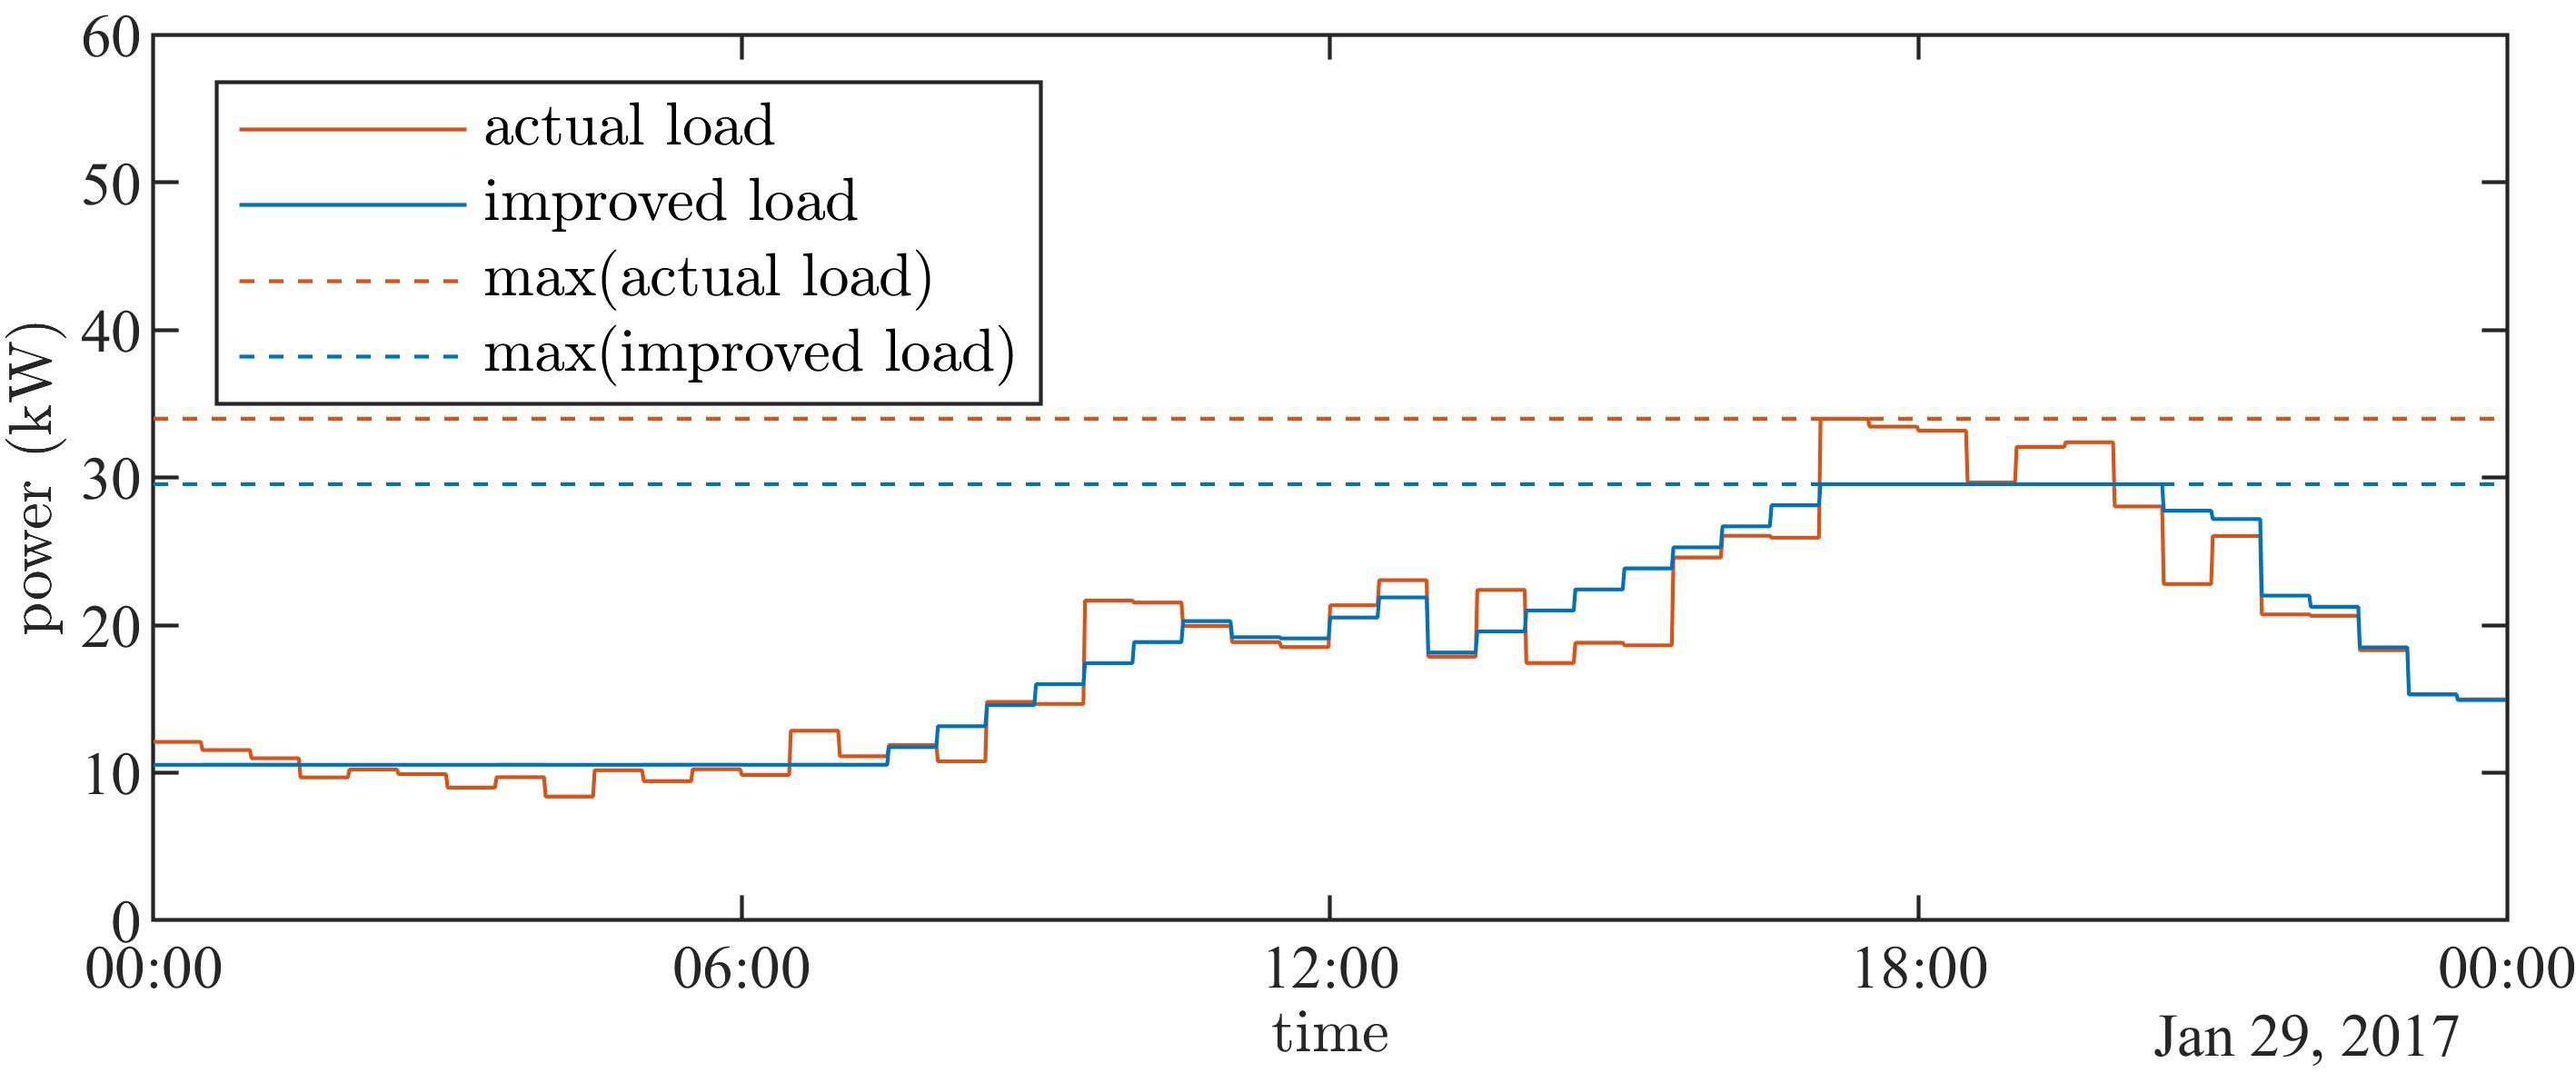
\includegraphics{_chapter2/fig/day-forecasted}
		\label{ch2:subfig:day-forecasted}
	}\\
	\subfloat[]{%
		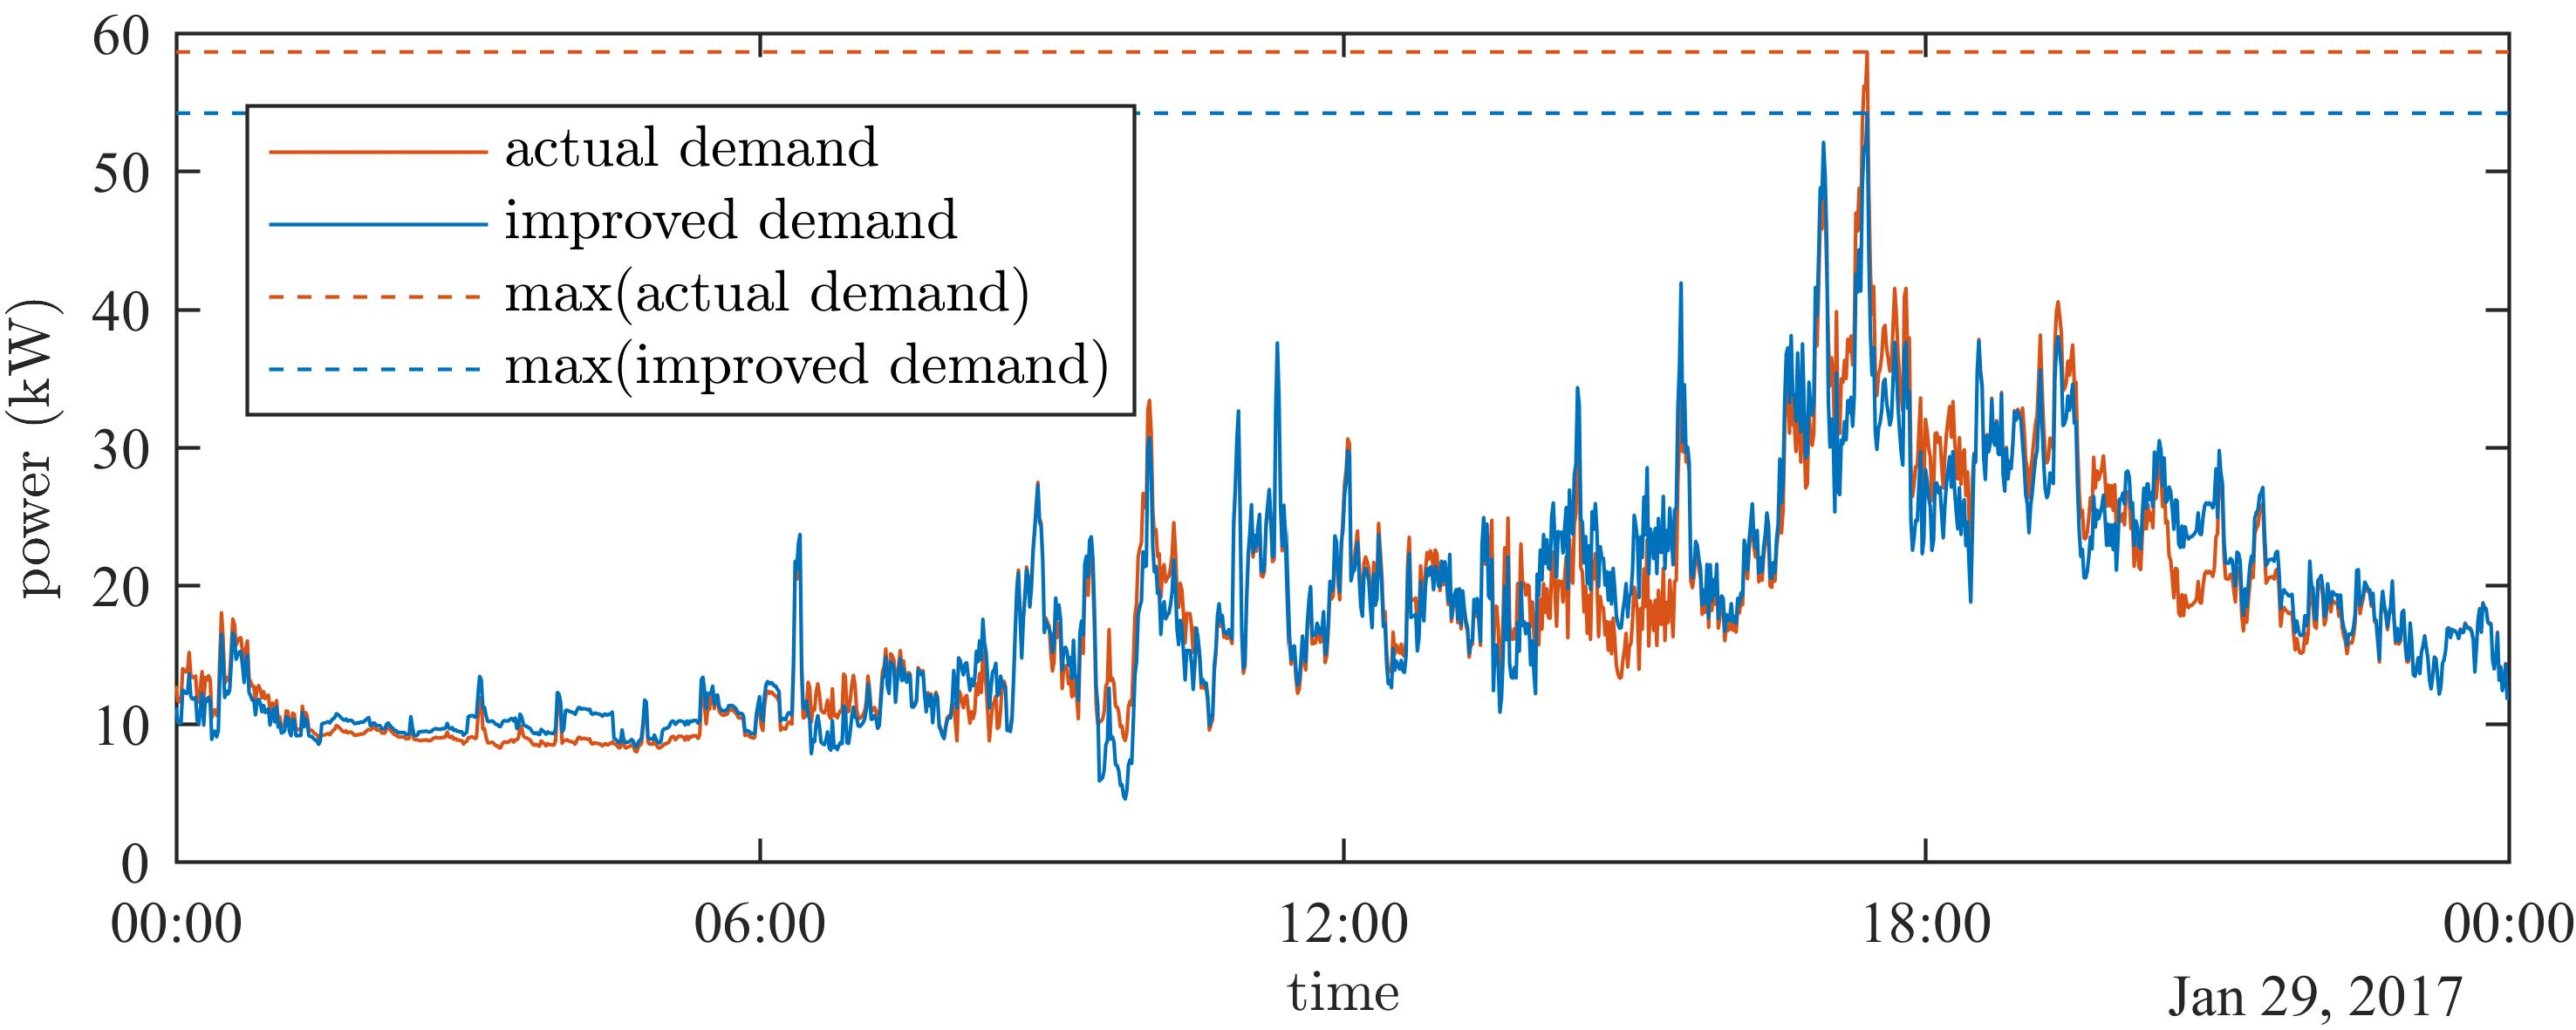
\includegraphics{_chapter2/fig/day-actual}
		\label{ch2:subfig:actual-forecasted}
	}
	\caption{An example of applying a half-hourly ESMU schedule to the half-hourly substation load (Subfig. \ref{ch2:subfig:day-forecasted}) and the actual, sub-half-hourly daily load, measured at the substation (Subfig. \ref{ch2:subfig:actual-forecasted}).}
	\label{ch2:fig:cost-sample}
\end{figure}

To visualise this schedule optimisation, a singe day's BESS schedule was generated from its forecast by using the cost minimisation as defined in Equation \ref{ch2:equ:cost-minimisation}.
When comparing the impact of the BESS schedule on to the actual sub-half-hourly demand, a noticeable disparity in peak duration, magnitude and volatility can be noted.
This disparity, as shown in Figure \ref{ch2:fig:cost-sample}, highlights the incompatibility issues between half-hourly BESS schedules and the actual sub-half-hourly load.
As previously discussed, benefits of BESS were intended to mitigate high-resolution volatility, yet this cannot be achieved when solely applying BESS schedules in an off-line manner.
Therefore, in the next section, the control strategy to add an on-line component is explained.




 